% Draft. Compile on Overleaf (IEEEtran is built in): pdflatex main; bibtex main; pdflatex main x2.
% Before submission: verify refs.bib, add author names/affiliations, check the venue's page limit and template.
\documentclass[conference]{IEEEtran}
\usepackage{graphicx,booktabs,amsmath,amssymb,multirow,url}
\usepackage[hidelinks]{hyperref}

\begin{document}

\title{Calibrating an EEG Foundation Model: A Controlled Re-evaluation of Neuro-GPT for Cross-Subject and Session-to-Session Motor Imagery Decoding}

\author{\IEEEauthorblockN{Author One, Author Two}
\IEEEauthorblockA{Department, Institution\\ email@institution}}

\maketitle

\begin{abstract}
EEG foundation models pre-trained with self-supervision promise to overcome the small size and heterogeneity of
brain-computer interface (BCI) datasets. We present a controlled re-evaluation of Neuro-GPT, an EEG encoder plus GPT
model pre-trained on the TUH EEG corpus, on 4-class motor imagery (BCI Competition IV-2a). First, we reproduce its best
fine-tuning recipe under leave-one-subject-out (LOSO) evaluation (0.600--0.607 vs.\ the reported 0.645) and show that the
public training script computes its final ``test'' metric on training subjects. Second, we test four ways to improve
cross-subject accuracy, selecting all settings on training subjects only: class-conditional soft prompt-tuning of the
frozen model, per-session Euclidean alignment, data augmentation and seed ensembling. None reliably improves on the
original recipe (best: $+0.022$, $p=0.13$). A linear-probe diagnostic explains the prompt-tuning failure: the frozen GPT's
output retains little class information (probe accuracy 0.356 vs.\ 0.493 for the encoder output, mean inter-sample
cosine similarity 0.97). Third, under the session-to-session protocol of the competition, calibrating the cross-subject
model on the target user's first session raises next-session accuracy from 0.588 to 0.711 (8 of 9 users improve);
an exploratory variant with per-session alignment in both stages reaches 0.754 and improves all 9 users. We
also document a case of negative transfer across sessions that a same-session validation split cannot detect. Code and
per-subject results are public.
\end{abstract}

\begin{IEEEkeywords}
EEG, foundation model, brain-computer interface, motor imagery, transfer learning, calibration, reproducibility
\end{IEEEkeywords}

\section{Introduction}
Deep EEG decoders suffer from small datasets and strong variability across subjects and sessions. Self-supervised
pre-training on large unlabeled corpora is a natural remedy, and Neuro-GPT~\cite{cui2024neurogpt} reported that a
pre-trained EEG encoder improves 4-class motor imagery decoding under LOSO evaluation (0.645 vs.\ 0.606 from scratch).
Such results are often reported on one split protocol, with one seed, and without statistical tests, which makes it
hard to know what actually drives performance and where the limits are.

We re-evaluate Neuro-GPT with a strictly controlled protocol and ask: (i) does the published recipe reproduce;
(ii) can parameter-efficient adaptation or standard cross-subject techniques raise LOSO accuracy; and (iii) how does
the model behave when a small amount of labeled data from the target user is available, as in practical BCIs?

\textbf{Contributions.}
\begin{itemize}
\item A reproduction of the encoder-only recipe on two machines, with a correction of the evaluation in the public code
(Sec.~\ref{sec:repro}).
\item A diagnosed negative result for class-conditional soft prompt-tuning of the frozen model, including a probe
showing that the frozen GPT discards class information (Sec.~\ref{sec:prompt}).
\item A training-subject-only selection study of alignment, augmentation and ensembling (Sec.~\ref{sec:levers}).
\item A session-to-session calibration study showing a large gain from cross-subject pre-adaptation, and a
documented case of cross-session negative transfer (Sec.~\ref{sec:calib}).
\end{itemize}

\section{Background: Neuro-GPT}
Neuro-GPT splits an EEG recording into $N$ chunks $D_1,\dots,D_N$ of $C\times T$ samples. An EEG Conformer
encoder~\cite{song2023conformer} (temporal convolution $1\times25$, spatial convolution $C\times1$, average pooling,
six self-attention layers) maps each chunk to a 1080-dimensional token $\mathcal{H}(D_i)$, projected to 1024 dimensions
for a six-layer GPT-2~\cite{radford2019gpt2}. Pre-training on 5,656 hours of TUH EEG~\cite{obeid2016tuh} uses causal
masking: in the $i$-th copy of the sequence the $i$-th token is replaced by a learnable mask token and later tokens are
zeroed, and the GPT output $\hat{Y}_i$ at the masked position is regressed onto the encoder embedding,
\begin{equation}
\mathcal{L} = \frac{1}{N-1}\sum_{i=2}^{N}\big\lVert \hat{Y}_i - \mathcal{H}(D_i)\big\rVert_2^2 .
\end{equation}
For BCI Competition IV-2a~\cite{brunner2008bci2a} (9 subjects, 22 channels, 250\,Hz, 288 trials per session, two
sessions) the data are mapped to the pre-training montage with a $22\times22$ source-space transform, and each trial
uses $t=2$--$6$\,s as two 2-s chunks. Of three fine-tuning strategies, \emph{encoder-only} (GPT discarded downstream)
was best.

\section{Experimental Protocol}
\textbf{Cross-subject (LOSO).} Fold $k$ trains on 8 subjects (both sessions) and tests on subject $k$. \textbf{Session-to-session.}
For each subject, train on session T and test on session E (another day); this uses target labels and is \emph{not}
comparable to LOSO. \textbf{Metric.} Accuracy at the final training step on held-out data; we never select checkpoints
on test data. \textbf{Recipe.} Authors' encoder-only fine-tuning: AdamW, lr $10^{-4}$, weight decay 0.1, linear schedule,
batch 32, 10,000 steps (5,000 where stated). \textbf{Selection.} Hyper-parameters are chosen on an inner split of the
training subjects of fold 0 (A02+A03 validate, A04--A09 train, A01 excluded), with decision rules fixed before results.
\textbf{Statistics.} Mean $\pm$ sample std over subjects; paired $t$-test and Wilcoxon signed-rank test across subjects.

\section{Results}
\subsection{Reproduction and an evaluation correction}\label{sec:repro}
In decoding mode, the public script evaluates its final ``test'' metric on the training subjects (on fold 0: 0.894,
vs.\ 0.648 on the held-out subject). Using held-out accuracy, the recipe gives $0.607\pm0.114$ (Colab T4) and
$0.600\pm0.113$ (RTX 3050), vs.\ $0.645\pm0.104$ reported. Training accuracy ($\approx$0.89) far exceeds held-out
accuracy, indicating that cross-subject shift, not capacity, limits performance.

\subsection{Soft prompt-tuning of the frozen model}\label{sec:prompt}
Following prompt tuning~\cite{lester2021prompt,li2021prefix}, we prepend a bank $P\in\mathbb{R}^{K\times m\times d}$
($K{=}4$ classes, $m{=}4$, $d{=}1024$) to every GPT input, freeze encoder and GPT, and train the bank, pooler and head
(1.34M of 78.7M parameters; note the encoder has only 0.16M). The original readout never learned (training loss at
$\ln 4$). A linear probe on fold 0 (Table~\ref{tab:probe}) shows that class information survives in the encoder output but
not in the frozen GPT's last-token state, which is nearly identical across trials. We also found that keeping frozen
modules in training mode (dropout $p{=}0.5$, BatchNorm updates) corrupts the features seen by the head; frozen modules
must be kept in evaluation mode. With these fixes and a trainable skip from the encoder, prompts did not help on the
folds completed (0.359 with vs.\ 0.357 without prompts, 4 folds).

\begin{table}[t]\centering\caption{Linear probe on frozen features (fold 0, test subject A01).}\label{tab:probe}
\begin{tabular}{lcc}\toprule
Features & Probe accuracy & Mean cosine \\ \midrule
EEG encoder output & 0.493 & 0.887 \\
GPT last-token state & 0.356 & 0.972 \\ \bottomrule
\end{tabular}\end{table}

\subsection{Alignment, augmentation and ensembling}\label{sec:levers}
Per-session Euclidean alignment~\cite{he2020ea} whitens each session by its mean covariance,
$R=\frac{1}{nT}\sum_i X_iX_i^\top$, $\tilde{X}_i=R^{-1/2}X_i$, using no labels. On all 9 folds it gives
$0.622\pm0.128$ vs.\ $0.600\pm0.113$ ($+0.022$, 5/9 subjects, $p=0.13$; Fig.~\ref{fig:loso}). On the inner split
(Table~\ref{tab:levers}) random cropping and noise augmentation reduced accuracy, and alignment did not pass the
pre-declared $+0.01$ threshold. Averaging the softmax outputs of three seeds gave $0.604$ vs.\ $0.599$ for single runs
($+0.005$, 8/9 subjects, $p=0.02$): consistent but small.

\begin{table}[t]\centering\caption{Inner-split validation accuracy (training subjects only).}\label{tab:levers}
\begin{tabular}{lc}\toprule
Setting & Accuracy \\ \midrule
Authors' recipe & \textbf{0.579} \\
Random crop $\pm$0.5\,s & 0.570 \\
Random crop $\pm$1\,s & 0.478 \\
$\pm$1\,s + noise + channel dropout + amplitude & 0.440 \\
Per-session alignment & 0.571 \\ \bottomrule
\end{tabular}\end{table}

\begin{figure}[t]\centering
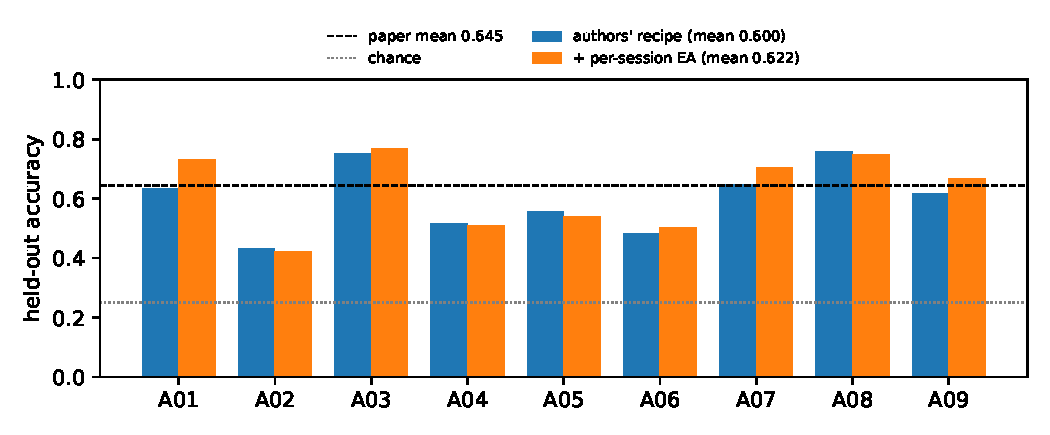
\includegraphics[width=\columnwidth]{figures/fig_cross_subject.pdf}
\caption{LOSO accuracy per held-out subject with and without per-session alignment.}\label{fig:loso}
\end{figure}

\subsection{Session-to-session calibration}\label{sec:calib}
Table~\ref{tab:calib} and Fig.~\ref{fig:calib} compare, on each subject's session E: the LOSO model without calibration;
the pre-trained model fine-tuned on session T only; and the LOSO model fine-tuned on session T (1,000 steps,
lr $5\times10^{-5}$, fixed in advance; 3 seeds). Cross-subject pre-adaptation followed by calibration reaches
$0.711\pm0.181$, improving 8 of 9 users over the LOSO model (Wilcoxon $p=0.055$). Subject A05 is a consistent exception
(0.29--0.35 in all seeds vs.\ $\approx$0.60 when calibrating from the pre-trained model alone). A validation-gated variant,
which picks per user among calibration candidates using 20\% of session T, scored 0.696: A05's model validates well within
session T (0.701) yet fails on session E (0.288), so this negative transfer arises between sessions and is invisible to a
same-session split. In an exploratory follow-up motivated by this case (and therefore partly fitted to the test
sessions), we applied per-session alignment in both stages: the LOSO model is trained on aligned data and calibrated on
aligned session T. This raised A05 to 0.717 (0.70--0.75 across seeds) and the mean to $0.754\pm0.101$, better than no
calibration for all 9 users (Wilcoxon $p=0.004$) but not significantly better than plain calibration ($+0.043$, 6/9,
$p=0.31$). A pre-registered replication on other datasets is needed to confirm it.

\begin{table}[t]\centering\caption{Session-E accuracy (mean $\pm$ std over 9 subjects, 3 seeds).}\label{tab:calib}
\begin{tabular}{lc}\toprule
Setting & Accuracy \\ \midrule
LOSO model, no calibration & $0.588\pm0.119$ \\
Pre-trained, fine-tuned on own session T & $0.622\pm0.091$ \\
LOSO model, fine-tuned on own session T & $\mathbf{0.711\pm0.181}$ \\
Validation-gated (80\% of T) & $0.696\pm0.189$ \\
Alignment in both stages (exploratory) & $0.754\pm0.101$ \\
\bottomrule
\end{tabular}\end{table}

\begin{figure}[t]\centering
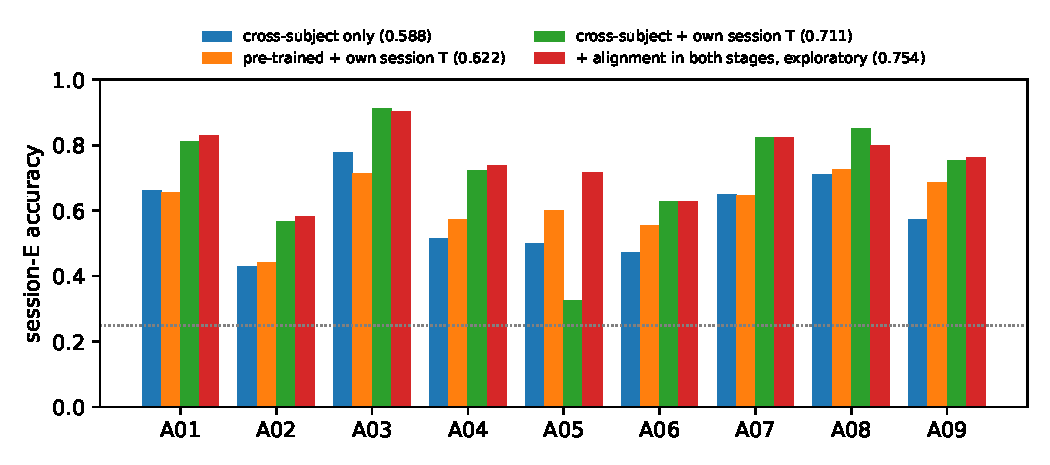
\includegraphics[width=\columnwidth]{figures/fig_calibration.pdf}
\caption{Session-E accuracy per subject for the calibration settings (the last bar is exploratory).}\label{fig:calib}
\end{figure}

\section{Discussion}
Cross-subject accuracy of Neuro-GPT appears bounded by inter-subject variability rather than by tuning: the gap between
training and held-out subjects is large, and alignment, augmentation, ensembling and prompt-tuning all fail to close it.
The probe offers a mechanistic reason why the GPT is discarded downstream in the original work and why prompt-tuning
the frozen GPT cannot help. When a single calibration session is available, the same model becomes much more useful, and
starting from a cross-subject model is better than starting from the pre-trained model for 8 of 9 users. The A05 case
shows that cross-subject pre-adaptation can also hurt, and that detecting this requires data from a later session.

\textbf{Limitations.} One dataset with 9 subjects; few seeds; the prompt-tuning study covers 4 folds; our reproduction is
$\approx$4 points below the reported mean; alignment is transductive for the test subject; we did not run a from-scratch
control; calibration settings were not tuned, which is conservative but may underestimate achievable accuracy.

\section{Conclusion}
A controlled re-evaluation of Neuro-GPT shows that its LOSO performance is hard to improve with prompt-tuning, alignment,
augmentation or ensembling, explains why with a probe of the frozen model, and shows that calibration on one session of
the target user raises next-session accuracy from 0.588 to 0.711 (0.754 in an exploratory variant with per-session alignment). We release code and per-subject results to support
further evaluation of EEG foundation models.

\section*{Code and Data Availability}
Code, scripts and per-subject results: \url{https://github.com/mir4gee/NeuroGPT}. BCI Competition IV-2a is public;
Neuro-GPT weights are released by the original authors.

\bibliographystyle{IEEEtran}
\bibliography{refs}
\end{document}
